\chapter{Experiments}
To show the usefulness of our improvements of the automatic generator, we have compared several solvers of some minimal problems using different methods in the automatic generator. We have used the benchmark of the automatic generator to generate the solvers and to compare the results because this tool is designed to it perfectly.

We have divided the experiments into three parts. In each part, we are comparing easily comparable methods on which the speed up of the new implemented method can be straightforwardly seen. In the first section, we are comparing one elimination solvers against multiple elimination solvers. In the second part, we are comparing solvers without the matrix partitioning used, with matrix partitioning used only to the last elimation and solvers with matrix partitioning used to all eliminations in the solver. In the last section, we are comparing solvers with different strategies of polynomial generation used. One solver is generated by the systematical generator and the second one is using the $F_4$ strategy.

We have choosen the 9-point relative pose different radial distortion problem \cite{9pt} for the testing. This problem consists of four polynomial equations in four unknowns. The number of all parameters is 63. The definition of this minimal problem can be found under the name \texttt{ku9pt} in the folder \texttt{minimalProblems} in the automatic generator. To generate the solvers, we have used the default settings of the automatic generator obtained by calling of the function \textit{gbs\_InitConfig} if not specified differently. We have tested the generated solvers on randomly generated data, but the data remained the same within each experiment. Each solver was tried on $1\,000$ instances of parameters. All test were performed on Intel Xeon E5-2630 2.30 GHz based computer. The MATLAB R2014a 64-bit was used to the tests.

\section{Multiple elimination solver}
In this part, we are comparing one elimination solver with multiple elimination solvers. We have generated one solver according to the description in the section \ref{subsec:polynomialGenerator}. This first solver consist only of one elimination in the end. The second and the third solvers have been generated as explained in the section \ref{subsec:multipleSolver}. The second solver has been generated with the variable $step$ set to 1 therefore, an elimination is performed always when the maximal total degree of the generated polynomials is increased by 1. This second solver consist of four Gauss-Jordan eliminations. The third solver has been generated with the variable $step$ set to 2. This means, that an elimination is performed when the maximal total degree of the generated polynomials is increased by 2. This solver consists of two eliminations.

We have used the benchmark templates specified in the function \textit{bench\_elimination} from the folder \texttt{benchmark} in the automatic generator. All other settings have remained default.

The computing times of these solvers are in the Table \ref{tab:elim}. The numerical stability of the solvers is shown in the Figure \ref{graph:elim} as histogram of $\log_{10}$ of absolute values of errors.

\begin{figure}[ht]
  \centering
  \resizebox{0.95\textwidth}{!}{% GNUPLOT: LaTeX picture with Postscript
\begingroup
  \makeatletter
  \providecommand\color[2][]{%
    \GenericError{(gnuplot) \space\space\space\@spaces}{%
      Package color not loaded in conjunction with
      terminal option `colourtext'%
    }{See the gnuplot documentation for explanation.%
    }{Either use 'blacktext' in gnuplot or load the package
      color.sty in LaTeX.}%
    \renewcommand\color[2][]{}%
  }%
  \providecommand\includegraphics[2][]{%
    \GenericError{(gnuplot) \space\space\space\@spaces}{%
      Package graphicx or graphics not loaded%
    }{See the gnuplot documentation for explanation.%
    }{The gnuplot epslatex terminal needs graphicx.sty or graphics.sty.}%
    \renewcommand\includegraphics[2][]{}%
  }%
  \providecommand\rotatebox[2]{#2}%
  \@ifundefined{ifGPcolor}{%
    \newif\ifGPcolor
    \GPcolorfalse
  }{}%
  \@ifundefined{ifGPblacktext}{%
    \newif\ifGPblacktext
    \GPblacktexttrue
  }{}%
  % define a \g@addto@macro without @ in the name:
  \let\gplgaddtomacro\g@addto@macro
  % define empty templates for all commands taking text:
  \gdef\gplbacktext{}%
  \gdef\gplfronttext{}%
  \makeatother
  \ifGPblacktext
    % no textcolor at all
    \def\colorrgb#1{}%
    \def\colorgray#1{}%
  \else
    % gray or color?
    \ifGPcolor
      \def\colorrgb#1{\color[rgb]{#1}}%
      \def\colorgray#1{\color[gray]{#1}}%
      \expandafter\def\csname LTw\endcsname{\color{white}}%
      \expandafter\def\csname LTb\endcsname{\color{black}}%
      \expandafter\def\csname LTa\endcsname{\color{black}}%
      \expandafter\def\csname LT0\endcsname{\color[rgb]{1,0,0}}%
      \expandafter\def\csname LT1\endcsname{\color[rgb]{0,1,0}}%
      \expandafter\def\csname LT2\endcsname{\color[rgb]{0,0,1}}%
      \expandafter\def\csname LT3\endcsname{\color[rgb]{1,0,1}}%
      \expandafter\def\csname LT4\endcsname{\color[rgb]{0,1,1}}%
      \expandafter\def\csname LT5\endcsname{\color[rgb]{1,1,0}}%
      \expandafter\def\csname LT6\endcsname{\color[rgb]{0,0,0}}%
      \expandafter\def\csname LT7\endcsname{\color[rgb]{1,0.3,0}}%
      \expandafter\def\csname LT8\endcsname{\color[rgb]{0.5,0.5,0.5}}%
    \else
      % gray
      \def\colorrgb#1{\color{black}}%
      \def\colorgray#1{\color[gray]{#1}}%
      \expandafter\def\csname LTw\endcsname{\color{white}}%
      \expandafter\def\csname LTb\endcsname{\color{black}}%
      \expandafter\def\csname LTa\endcsname{\color{black}}%
      \expandafter\def\csname LT0\endcsname{\color{black}}%
      \expandafter\def\csname LT1\endcsname{\color{black}}%
      \expandafter\def\csname LT2\endcsname{\color{black}}%
      \expandafter\def\csname LT3\endcsname{\color{black}}%
      \expandafter\def\csname LT4\endcsname{\color{black}}%
      \expandafter\def\csname LT5\endcsname{\color{black}}%
      \expandafter\def\csname LT6\endcsname{\color{black}}%
      \expandafter\def\csname LT7\endcsname{\color{black}}%
      \expandafter\def\csname LT8\endcsname{\color{black}}%
    \fi
  \fi
  \setlength{\unitlength}{0.0500bp}%
  \begin{picture}(8640.00,5040.00)%
    \gplgaddtomacro\gplbacktext{%
      \csname LTb\endcsname%
      \put(814,704){\makebox(0,0)[r]{\strut{} 0}}%
      \csname LTb\endcsname%
      \put(814,1286){\makebox(0,0)[r]{\strut{} 2}}%
      \csname LTb\endcsname%
      \put(814,1867){\makebox(0,0)[r]{\strut{} 4}}%
      \csname LTb\endcsname%
      \put(814,2449){\makebox(0,0)[r]{\strut{} 6}}%
      \csname LTb\endcsname%
      \put(814,3030){\makebox(0,0)[r]{\strut{} 8}}%
      \csname LTb\endcsname%
      \put(814,3612){\makebox(0,0)[r]{\strut{} 10}}%
      \csname LTb\endcsname%
      \put(814,4193){\makebox(0,0)[r]{\strut{} 12}}%
      \csname LTb\endcsname%
      \put(814,4775){\makebox(0,0)[r]{\strut{} 14}}%
      \csname LTb\endcsname%
      \put(946,484){\makebox(0,0){\strut{}-14}}%
      \csname LTb\endcsname%
      \put(1676,484){\makebox(0,0){\strut{}-12}}%
      \csname LTb\endcsname%
      \put(2405,484){\makebox(0,0){\strut{}-10}}%
      \csname LTb\endcsname%
      \put(3135,484){\makebox(0,0){\strut{}-8}}%
      \csname LTb\endcsname%
      \put(3865,484){\makebox(0,0){\strut{}-6}}%
      \csname LTb\endcsname%
      \put(4595,484){\makebox(0,0){\strut{}-4}}%
      \csname LTb\endcsname%
      \put(5324,484){\makebox(0,0){\strut{}-2}}%
      \csname LTb\endcsname%
      \put(6054,484){\makebox(0,0){\strut{} 0}}%
      \csname LTb\endcsname%
      \put(6784,484){\makebox(0,0){\strut{} 2}}%
      \csname LTb\endcsname%
      \put(7513,484){\makebox(0,0){\strut{} 4}}%
      \csname LTb\endcsname%
      \put(8243,484){\makebox(0,0){\strut{} 6}}%
      \put(176,2739){\rotatebox{-270}{\makebox(0,0){\strut{}Frequency}}}%
      \put(4594,154){\makebox(0,0){\strut{}log$_{10}$($|$error$|$)}}%
      \put(4594,4665){\makebox(0,0){\strut{}}}%
    }%
    \gplgaddtomacro\gplfronttext{%
      \csname LTb\endcsname%
      \put(7256,4602){\makebox(0,0)[r]{\strut{}Without matrix partitioning}}%
      \csname LTb\endcsname%
      \put(7256,4382){\makebox(0,0)[r]{\strut{}Last elimination with matrix partitioning}}%
      \csname LTb\endcsname%
      \put(7256,4162){\makebox(0,0)[r]{\strut{}All eliminations with matrix partitioning}}%
    }%
    \gplbacktext
    \put(0,0){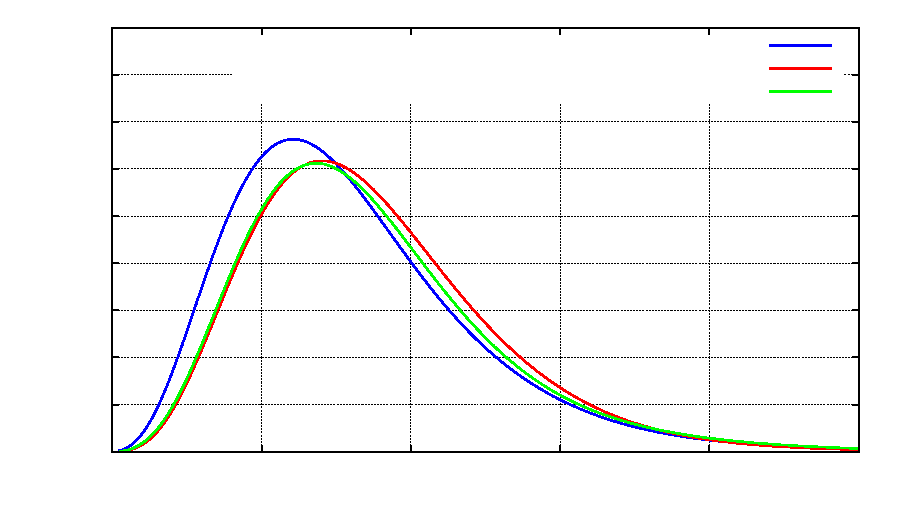
\includegraphics{graphs/elim}}%
    \gplfronttext
  \end{picture}%
\endgroup
}
  \caption{Histogram of $\log_{10}$ of absolute values of errors for one elimination and multiple elimination solvers.}
  \label{graph:elim}
\end{figure}

\begin{table}[ht]
  \centering
  \begin{tabular}{|c||ccc|}
    \hline
      & \textbf{One elimination} & \textbf{Multiple elimination} & \textbf{Multiple elimination} \\
      & \textbf{solver}          & \textbf{solver} ($step = 1$)  & \textbf{solver} ($step = 2$)\\
    \hline\hline
    \textbf{minimal} & 1.988 & 1.036 & 1.745\\
\textbf{median} & 2.799 & 2.003 & 2.198\\
\textbf{maximal} & 2.859 & 2.227 & 2.283\\

    \hline
  \end{tabular}
  \caption{Computing times of one and multiple elimination solvers.}
  \label{tab:elim}
\end{table}

You can see that the numerical stability of the multiple elimination solvers is slightly worse than the numerical stability of the one elimination solver. In the contrary, the multi elimination solvers are approximately 1.5 times faster than the one elimination solver. Interesting is that the second and third solvers are equivalently fast, but one of them consists of four eliminations and the second one only of two eliminations. Therefore, we can not say that more eliminations lead to faster solvers. So, it is important to run the benchmark to find the optimal number of eliminations for each minimal problem and then choose the best solver for the application.

\section{Matrix partitioning}
\begin{figure}[ht]
  \centering
  \resizebox{0.95\textwidth}{!}{% GNUPLOT: LaTeX picture with Postscript
\begingroup
  \makeatletter
  \providecommand\color[2][]{%
    \GenericError{(gnuplot) \space\space\space\@spaces}{%
      Package color not loaded in conjunction with
      terminal option `colourtext'%
    }{See the gnuplot documentation for explanation.%
    }{Either use 'blacktext' in gnuplot or load the package
      color.sty in LaTeX.}%
    \renewcommand\color[2][]{}%
  }%
  \providecommand\includegraphics[2][]{%
    \GenericError{(gnuplot) \space\space\space\@spaces}{%
      Package graphicx or graphics not loaded%
    }{See the gnuplot documentation for explanation.%
    }{The gnuplot epslatex terminal needs graphicx.sty or graphics.sty.}%
    \renewcommand\includegraphics[2][]{}%
  }%
  \providecommand\rotatebox[2]{#2}%
  \@ifundefined{ifGPcolor}{%
    \newif\ifGPcolor
    \GPcolorfalse
  }{}%
  \@ifundefined{ifGPblacktext}{%
    \newif\ifGPblacktext
    \GPblacktexttrue
  }{}%
  % define a \g@addto@macro without @ in the name:
  \let\gplgaddtomacro\g@addto@macro
  % define empty templates for all commands taking text:
  \gdef\gplbacktext{}%
  \gdef\gplfronttext{}%
  \makeatother
  \ifGPblacktext
    % no textcolor at all
    \def\colorrgb#1{}%
    \def\colorgray#1{}%
  \else
    % gray or color?
    \ifGPcolor
      \def\colorrgb#1{\color[rgb]{#1}}%
      \def\colorgray#1{\color[gray]{#1}}%
      \expandafter\def\csname LTw\endcsname{\color{white}}%
      \expandafter\def\csname LTb\endcsname{\color{black}}%
      \expandafter\def\csname LTa\endcsname{\color{black}}%
      \expandafter\def\csname LT0\endcsname{\color[rgb]{1,0,0}}%
      \expandafter\def\csname LT1\endcsname{\color[rgb]{0,1,0}}%
      \expandafter\def\csname LT2\endcsname{\color[rgb]{0,0,1}}%
      \expandafter\def\csname LT3\endcsname{\color[rgb]{1,0,1}}%
      \expandafter\def\csname LT4\endcsname{\color[rgb]{0,1,1}}%
      \expandafter\def\csname LT5\endcsname{\color[rgb]{1,1,0}}%
      \expandafter\def\csname LT6\endcsname{\color[rgb]{0,0,0}}%
      \expandafter\def\csname LT7\endcsname{\color[rgb]{1,0.3,0}}%
      \expandafter\def\csname LT8\endcsname{\color[rgb]{0.5,0.5,0.5}}%
    \else
      % gray
      \def\colorrgb#1{\color{black}}%
      \def\colorgray#1{\color[gray]{#1}}%
      \expandafter\def\csname LTw\endcsname{\color{white}}%
      \expandafter\def\csname LTb\endcsname{\color{black}}%
      \expandafter\def\csname LTa\endcsname{\color{black}}%
      \expandafter\def\csname LT0\endcsname{\color{black}}%
      \expandafter\def\csname LT1\endcsname{\color{black}}%
      \expandafter\def\csname LT2\endcsname{\color{black}}%
      \expandafter\def\csname LT3\endcsname{\color{black}}%
      \expandafter\def\csname LT4\endcsname{\color{black}}%
      \expandafter\def\csname LT5\endcsname{\color{black}}%
      \expandafter\def\csname LT6\endcsname{\color{black}}%
      \expandafter\def\csname LT7\endcsname{\color{black}}%
      \expandafter\def\csname LT8\endcsname{\color{black}}%
    \fi
  \fi
  \setlength{\unitlength}{0.0500bp}%
  \begin{picture}(8640.00,5040.00)%
    \gplgaddtomacro\gplbacktext{%
      \csname LTb\endcsname%
      \put(946,704){\makebox(0,0)[r]{\strut{} 0}}%
      \csname LTb\endcsname%
      \put(946,1156){\makebox(0,0)[r]{\strut{} 50}}%
      \csname LTb\endcsname%
      \put(946,1609){\makebox(0,0)[r]{\strut{} 100}}%
      \csname LTb\endcsname%
      \put(946,2061){\makebox(0,0)[r]{\strut{} 150}}%
      \csname LTb\endcsname%
      \put(946,2513){\makebox(0,0)[r]{\strut{} 200}}%
      \csname LTb\endcsname%
      \put(946,2966){\makebox(0,0)[r]{\strut{} 250}}%
      \csname LTb\endcsname%
      \put(946,3418){\makebox(0,0)[r]{\strut{} 300}}%
      \csname LTb\endcsname%
      \put(946,3870){\makebox(0,0)[r]{\strut{} 350}}%
      \csname LTb\endcsname%
      \put(946,4323){\makebox(0,0)[r]{\strut{} 400}}%
      \csname LTb\endcsname%
      \put(946,4775){\makebox(0,0)[r]{\strut{} 450}}%
      \csname LTb\endcsname%
      \put(1078,484){\makebox(0,0){\strut{}-15}}%
      \csname LTb\endcsname%
      \put(2511,484){\makebox(0,0){\strut{}-10}}%
      \csname LTb\endcsname%
      \put(3944,484){\makebox(0,0){\strut{}-5}}%
      \csname LTb\endcsname%
      \put(5377,484){\makebox(0,0){\strut{} 0}}%
      \csname LTb\endcsname%
      \put(6810,484){\makebox(0,0){\strut{} 5}}%
      \csname LTb\endcsname%
      \put(8243,484){\makebox(0,0){\strut{} 10}}%
      \put(176,2739){\rotatebox{-270}{\makebox(0,0){\strut{}Frequency}}}%
      \put(4660,154){\makebox(0,0){\strut{}log$_{10}\Big(\big|$error$\big|\Big)$}}%
      \put(4660,4665){\makebox(0,0){\strut{}}}%
    }%
    \gplgaddtomacro\gplfronttext{%
      \csname LTb\endcsname%
      \put(7256,4602){\makebox(0,0)[r]{\strut{}Without matrix partitioning}}%
      \csname LTb\endcsname%
      \put(7256,4382){\makebox(0,0)[r]{\strut{}Last elimination with matrix partitioning}}%
      \csname LTb\endcsname%
      \put(7256,4162){\makebox(0,0)[r]{\strut{}All eliminations with matrix partitioning}}%
    }%
    \gplbacktext
    \put(0,0){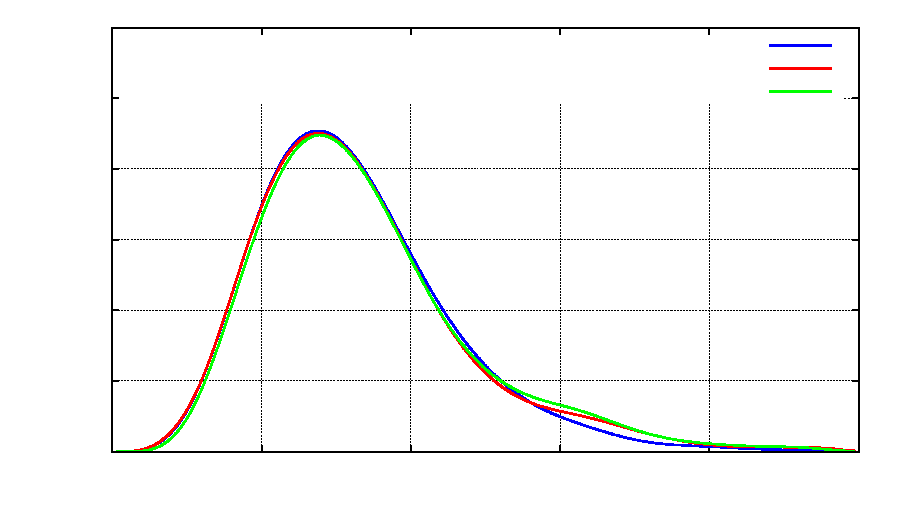
\includegraphics{graphs/part}}%
    \gplfronttext
  \end{picture}%
\endgroup
}
  \caption{Histogram of $\log_{10}$ of absolute values of errors for solver without matrix partitioning, solver with matrix partitioning only for the last elimination and solver with matrix partitioning for all eliminations in the solver.}
  \label{graph:part}
\end{figure}

\begin{table}[ht]
  \centering
  \begin{tabular}{|c||ccc|}
    \hline
      & \textbf{Without matrix} & \textbf{Matrix partitioning}      & \textbf{Matrix paritioning} \\
      & \textbf{partitioning}   & \textbf{for the last elimination} & \textbf{for all eliminations} \\
    \hline\hline
    \textbf{minimal time} & 1.353 s & 0.956 s & 0.794 s\\
\textbf{median of times} & 2.185 s & 1.071 s & 0.932 s\\
\textbf{maximal time} & 2.604 s & 1.189 s & 2.273 s\\

    \hline
  \end{tabular}
  \caption{Computing times of solver without matrix partitioning, of solver with matrix partitioning used for the last elimination and of solver with matrix partitioning used for all eliminations in the solver.}
  \label{tab:part}
\end{table}

\section{$F_4$ strategy}
\begin{figure}[ht]
  \centering
  \resizebox{0.95\textwidth}{!}{% GNUPLOT: LaTeX picture with Postscript
\begingroup
  \makeatletter
  \providecommand\color[2][]{%
    \GenericError{(gnuplot) \space\space\space\@spaces}{%
      Package color not loaded in conjunction with
      terminal option `colourtext'%
    }{See the gnuplot documentation for explanation.%
    }{Either use 'blacktext' in gnuplot or load the package
      color.sty in LaTeX.}%
    \renewcommand\color[2][]{}%
  }%
  \providecommand\includegraphics[2][]{%
    \GenericError{(gnuplot) \space\space\space\@spaces}{%
      Package graphicx or graphics not loaded%
    }{See the gnuplot documentation for explanation.%
    }{The gnuplot epslatex terminal needs graphicx.sty or graphics.sty.}%
    \renewcommand\includegraphics[2][]{}%
  }%
  \providecommand\rotatebox[2]{#2}%
  \@ifundefined{ifGPcolor}{%
    \newif\ifGPcolor
    \GPcolorfalse
  }{}%
  \@ifundefined{ifGPblacktext}{%
    \newif\ifGPblacktext
    \GPblacktexttrue
  }{}%
  % define a \g@addto@macro without @ in the name:
  \let\gplgaddtomacro\g@addto@macro
  % define empty templates for all commands taking text:
  \gdef\gplbacktext{}%
  \gdef\gplfronttext{}%
  \makeatother
  \ifGPblacktext
    % no textcolor at all
    \def\colorrgb#1{}%
    \def\colorgray#1{}%
  \else
    % gray or color?
    \ifGPcolor
      \def\colorrgb#1{\color[rgb]{#1}}%
      \def\colorgray#1{\color[gray]{#1}}%
      \expandafter\def\csname LTw\endcsname{\color{white}}%
      \expandafter\def\csname LTb\endcsname{\color{black}}%
      \expandafter\def\csname LTa\endcsname{\color{black}}%
      \expandafter\def\csname LT0\endcsname{\color[rgb]{1,0,0}}%
      \expandafter\def\csname LT1\endcsname{\color[rgb]{0,1,0}}%
      \expandafter\def\csname LT2\endcsname{\color[rgb]{0,0,1}}%
      \expandafter\def\csname LT3\endcsname{\color[rgb]{1,0,1}}%
      \expandafter\def\csname LT4\endcsname{\color[rgb]{0,1,1}}%
      \expandafter\def\csname LT5\endcsname{\color[rgb]{1,1,0}}%
      \expandafter\def\csname LT6\endcsname{\color[rgb]{0,0,0}}%
      \expandafter\def\csname LT7\endcsname{\color[rgb]{1,0.3,0}}%
      \expandafter\def\csname LT8\endcsname{\color[rgb]{0.5,0.5,0.5}}%
    \else
      % gray
      \def\colorrgb#1{\color{black}}%
      \def\colorgray#1{\color[gray]{#1}}%
      \expandafter\def\csname LTw\endcsname{\color{white}}%
      \expandafter\def\csname LTb\endcsname{\color{black}}%
      \expandafter\def\csname LTa\endcsname{\color{black}}%
      \expandafter\def\csname LT0\endcsname{\color{black}}%
      \expandafter\def\csname LT1\endcsname{\color{black}}%
      \expandafter\def\csname LT2\endcsname{\color{black}}%
      \expandafter\def\csname LT3\endcsname{\color{black}}%
      \expandafter\def\csname LT4\endcsname{\color{black}}%
      \expandafter\def\csname LT5\endcsname{\color{black}}%
      \expandafter\def\csname LT6\endcsname{\color{black}}%
      \expandafter\def\csname LT7\endcsname{\color{black}}%
      \expandafter\def\csname LT8\endcsname{\color{black}}%
    \fi
  \fi
  \setlength{\unitlength}{0.0500bp}%
  \begin{picture}(8640.00,5040.00)%
    \gplgaddtomacro\gplbacktext{%
      \csname LTb\endcsname%
      \put(946,704){\makebox(0,0)[r]{\strut{} 0}}%
      \csname LTb\endcsname%
      \put(946,1156){\makebox(0,0)[r]{\strut{} 100}}%
      \csname LTb\endcsname%
      \put(946,1609){\makebox(0,0)[r]{\strut{} 200}}%
      \csname LTb\endcsname%
      \put(946,2061){\makebox(0,0)[r]{\strut{} 300}}%
      \csname LTb\endcsname%
      \put(946,2513){\makebox(0,0)[r]{\strut{} 400}}%
      \csname LTb\endcsname%
      \put(946,2966){\makebox(0,0)[r]{\strut{} 500}}%
      \csname LTb\endcsname%
      \put(946,3418){\makebox(0,0)[r]{\strut{} 600}}%
      \csname LTb\endcsname%
      \put(946,3870){\makebox(0,0)[r]{\strut{} 700}}%
      \csname LTb\endcsname%
      \put(946,4323){\makebox(0,0)[r]{\strut{} 800}}%
      \csname LTb\endcsname%
      \put(946,4775){\makebox(0,0)[r]{\strut{} 900}}%
      \csname LTb\endcsname%
      \put(1078,484){\makebox(0,0){\strut{}-15}}%
      \csname LTb\endcsname%
      \put(2272,484){\makebox(0,0){\strut{}-10}}%
      \csname LTb\endcsname%
      \put(3466,484){\makebox(0,0){\strut{}-5}}%
      \csname LTb\endcsname%
      \put(4661,484){\makebox(0,0){\strut{} 0}}%
      \csname LTb\endcsname%
      \put(5855,484){\makebox(0,0){\strut{} 5}}%
      \csname LTb\endcsname%
      \put(7049,484){\makebox(0,0){\strut{} 10}}%
      \csname LTb\endcsname%
      \put(8243,484){\makebox(0,0){\strut{} 15}}%
      \put(176,2739){\rotatebox{-270}{\makebox(0,0){\strut{}Frequency}}}%
      \put(4660,154){\makebox(0,0){\strut{}log$_{10}$($|$error$|$)}}%
      \put(4660,4665){\makebox(0,0){\strut{}}}%
    }%
    \gplgaddtomacro\gplfronttext{%
      \csname LTb\endcsname%
      \put(7256,4602){\makebox(0,0)[r]{\strut{}Without matrix partitioning}}%
      \csname LTb\endcsname%
      \put(7256,4382){\makebox(0,0)[r]{\strut{}Last elimination with matrix partitioning}}%
    }%
    \gplbacktext
    \put(0,0){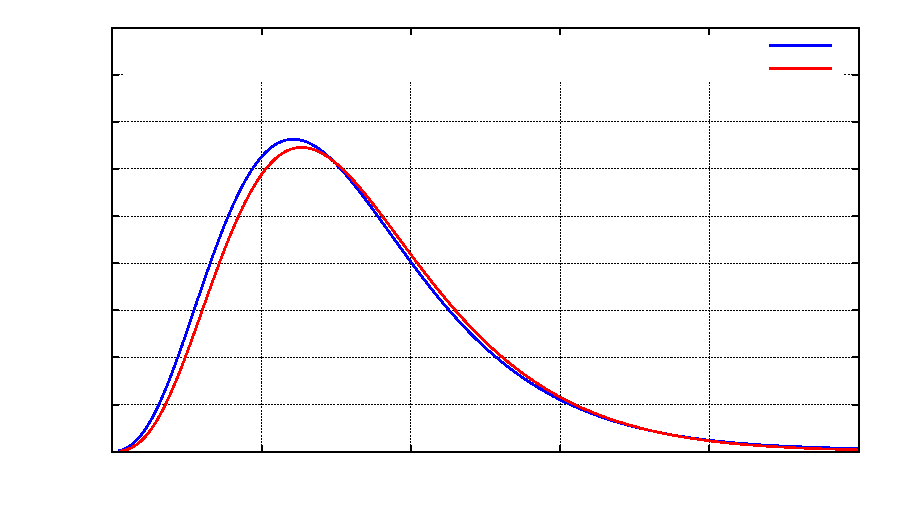
\includegraphics{graphs/gen}}%
    \gplfronttext
  \end{picture}%
\endgroup
}
  \caption{Histogram of $\log_{10}$ of absolute values of errors for solver generated by the systematical generator and for solver using the $F_4$ strategy.}
  \label{graph:gen}
\end{figure}

\begin{table}[ht]
  \centering
  \begin{tabular}{|c||cc|}
    \hline
    & \textbf{Systematical}    & \textbf{$F_4$ strategy} \\
    &  \textbf{generator used} & \textbf{used} \\
    \hline\hline
    \textbf{minimal} & 2.213 & 0.615\\
\textbf{median} & 2.895 & 0.713\\
\textbf{maximal} & 3.320 & 1.161\\

    \hline
  \end{tabular}
  \caption{Computing times of solver generated by the systematical generator and of the solver using the $F_4$ strategy.}
  \label{tab:gen}
\end{table}
